\documentclass[11pt,a4paper]{article}
\usepackage[utf8]{inputenc}
\usepackage[T1]{fontenc}
\usepackage{lmodern}
\usepackage[spanish,es-tabla]{babel}
\usepackage{amsmath,amssymb,mathtools}
\usepackage{booktabs,array,graphicx,float,xcolor,microtype,caption,enumitem,textcomp}
\newcommand{\euro}{\texteuro}
\usepackage[margin=2.5cm]{geometry}
\usepackage[hidelinks]{hyperref}
\captionsetup{font=small,labelfont=bf}
\newcommand{\E}{\mathbb{E}}
\newcommand{\Var}{\mathrm{Var}}
\newcommand{\Cov}{\mathrm{Cov}}
\title{\textbf{Tema 2 -- Preguntas de repaso}\\[2pt]\large Modelo individual del coste total de siniestralidad}
\author{Luiz Luzuriaga}
\date{M\'aster en Ciencias Actuariales y Financieras -- Universidad de Alcal\'a\\
Matem\'atica Actuarial de la Estabilidad y Solvencia de la Actividad Aseguradora\\ Curso 2026-27}
\begin{document}
\maketitle

\section*{Pregunta 1 -- Independientes pero no id\'enticamente distribuidas}

\noindent\textbf{Enunciado.} ?`Por qu\'e se afirma que las $X_i$ del modelo individual son independientes pero no id\'enticamente distribuidas? ?`Qu\'e implicaci\'on tiene esto para el c\'alculo de $\Var(S)$?

\subsection*{Por qu\'e no id\'enticas}
Cada p\'oliza es $X_i=I_iB_i$, con $I_i\sim\text{Bernoulli}(q_i)$ y severidad $B_i$ de media $\mu_i$ y varianza $\sigma_i^2$. Cada p\'oliza trae su propio vector $(q_i,\mu_i,\sigma_i^2)$: edad y sexo del asegurado, capital asegurado $b_i$, garant\'ias, zona, antig\"uedad. Dos p\'olizas con el mismo $q$ pero distinto capital ya tienen distribuciones distintas, as\'i que $S=\sum X_i$ no es una suma de copias de una misma variable. Esta es justamente la diferencia con el modelo colectivo, donde se supone que las cuant\'ias $Y_j$ son i.i.d.

\subsection*{Por qu\'e independientes}
Es una hip\'otesis de modelizaci\'on: el que una p\'oliza genere siniestro no altera la probabilidad de que lo genere otra (condicionando a lo que ya sabemos de cada una). Matem\'aticamente, $I_1,\dots,I_n,B_1,\dots,B_n$ son mutuamente independientes. Hace falta para que todo lo que sigue sea manejable.

\subsection*{Implicaciones sobre $\Var(S)$}
\begin{enumerate}[leftmargin=*]
\item \textbf{Se suman varianzas, no desviaciones t\'ipicas.} Con independencia todas las covarianzas son nulas y
\[
\Var(S)=\sum_{i=1}^n\Var(X_i)=\sum_{i=1}^n\Big[q_i\sigma_i^2+q_i(1-q_i)\mu_i^2\Big],\qquad SD(S)=\sqrt{\textstyle\sum_i\Var(X_i)}\ \ll\ \sum_i SD(X_i).
\]
Esa diferencia entre $\sqrt{\sum\Var}$ y $\sum SD$ es toda la \emph{ganancia de diversificaci\'on}.
\item \textbf{No id\'enticas $\Rightarrow$ no hay f\'ormula $n\,\Var(X)$.} La varianza hay que calcularla p\'oliza a p\'oliza (o por grupos homog\'eneos, donde s\'i valen $n_gq_g(1-q_g)b_g^2$). Tampoco se usa una Binomial \'unica para el n\'umero de siniestros: es una suma de Bernoullis con probabilidades distintas.
\item \textbf{La varianza se concentra en los capitales altos.} Como $\Var(X_i)=q_i(1-q_i)b_i^2$, la severidad entra \emph{al cuadrado}. En la cartera de 8 p\'olizas del taller, la p\'oliza 8 ($b=300.000$) aporta el $41{,}1\%$ de la prima pura esperada pero el $54{,}5\%$ de $\Var(S)$. En el Caso~1, el grupo D (50 p\'olizas, el $5\%$ del n\'umero) aporta el $38\%$ de la varianza con el $24{,}6\%$ de la prima esperada. Por eso la atenci\'on de suscripci\'on y reaseguro se dirige a los capitales altos.
\item \textbf{La independencia es lo que hace falta comprobar.} Si en vez de independientes hubiera correlaci\'on, $\Var(S)=\sum\Var(X_i)+\sum_{i\ne j}\Cov(X_i,X_j)$, y los t\'erminos cruzados son $n(n-1)$ frente a $n$ diagonales. Con una correlaci\'on constante $\rho$ entre los $X_i$: $\Var(S)=(1-\rho)\sum\Var(X_i)+\rho\big(\sum SD(X_i)\big)^2$. En el Caso~1, $\rho=0{,}001$ (una mil\'esima) multiplica la varianza por $1{,}67$ y lleva el VaR Normal de $1.491.844$ a $1.750.382$ \euro; con $\rho=0{,}01$ la varianza se multiplica por $7{,}7$. La independencia no es un detalle: es la hip\'otesis que m\'as pesa en el capital.
\item \textbf{Aproximaci\'on normal.} Como las $X_i$ no son id\'enticas no basta el TCL cl\'asico: se necesita la condici\'on de Lindeberg (que ninguna p\'oliza domine la suma). Una cartera con una p\'oliza gigante no converge a la Normal.
\end{enumerate}

\paragraph{Conclusi\'on.} ``Independientes'' permite sumar varianzas y diversificar; ``no id\'enticas'' obliga a calcularlas una a una y hace que el riesgo dependa de c\'omo se reparten los capitales, no solo de cu\'antas p\'olizas hay.

\bigskip\hrule\bigskip

\section*{Pregunta 2 -- Por qu\'e la Normal infravalora el capital}

\noindent\textbf{Enunciado.} Explica con tus palabras por qu\'e la aproximaci\'on Normal tiende a infravalorar el capital necesario en carteras de seguros.

\subsection*{Idea}
El capital se calcula con un cuantil muy alto (99,5\,\%), es decir, en la \emph{cola derecha}. La Normal es sim\'etrica; la siniestralidad agregada no lo es. El coeficiente de asimetr\'ia $\gamma_S=\mu_3(S)/\sigma_S^3$ es positivo porque hay muchos a\~nos con pocos siniestros y pocos a\~nos con muchos y grandes. Una Normal con la misma media y varianza reparte esa masa de forma sim\'etrica y deja la cola derecha demasiado ligera.

\subsection*{Por qu\'e la correcci\'on tiene ese signo: Edgeworth y Cornish--Fisher}
El teorema central del l\'imite garantiza convergencia a la Normal, pero la convergencia es buena en el centro y mala en las colas. El primer t\'ermino de correcci\'on (Edgeworth) es
\[
F_S(x)\approx\Phi(z)-\varphi(z)\,\frac{\gamma_S}{6}\,(z^2-1),\qquad z=\frac{x-\E[S]}{\sigma_S}.
\]
Para $z>1$ el factor $z^2-1$ es positivo y, con $\gamma_S>0$, la funci\'on de distribuci\'on real es \emph{menor} que $\Phi(z)$: queda m\'as probabilidad a la derecha. Invirtiendo, el cuantil verdadero es mayor que el Normal. Es la f\'ormula de Cornish--Fisher de primer orden, la \emph{Normal Power}:
\[
x_p\approx\E[S]+\sigma_S\Big[z_p+\frac{\gamma_S}{6}(z_p^2-1)\Big].
\]
La correcci\'on crece con $z_p^2$: es peque\~na al 90\,\% y grande al 99,5\,\%; por eso el error de la Normal se concentra justo en el nivel regulatorio.

\subsection*{Cuantificaci\'on con el Caso 1}
$\E[S]=610.000$, $SD=342.354$, $\gamma_S=0{,}627$, $z_{0{,}995}=2{,}576$. La correcci\'on es $0{,}627/6\cdot(2{,}576^2-1)=0{,}589$ desviaciones t\'ipicas, es decir $+201.630$ \euro. Resultado:
\begin{center}
\begin{tabular}{lrr}
\toprule
M\'etodo & VaR 99,5\,\% (\euro) & Capital sobre $\E[S]$ (\euro)\\
\midrule
Normal & 1.491.844 & 881.844\\
Gamma trasladada & 1.690.793 & 1.080.793\\
Normal Power & 1.693.480 & 1.083.480\\
Exacta (convoluci\'on) & 1.700.000 & 1.090.000\\
\bottomrule
\end{tabular}
\end{center}
La Normal deja un $12{,}2\%$ por debajo del exacto, y la probabilidad real de superar el ``VaR 99,5\,\%'' Normal no es $0{,}5\%$ sino $1{,}50\%$: tres veces mayor.
\begin{figure}[H]\centering
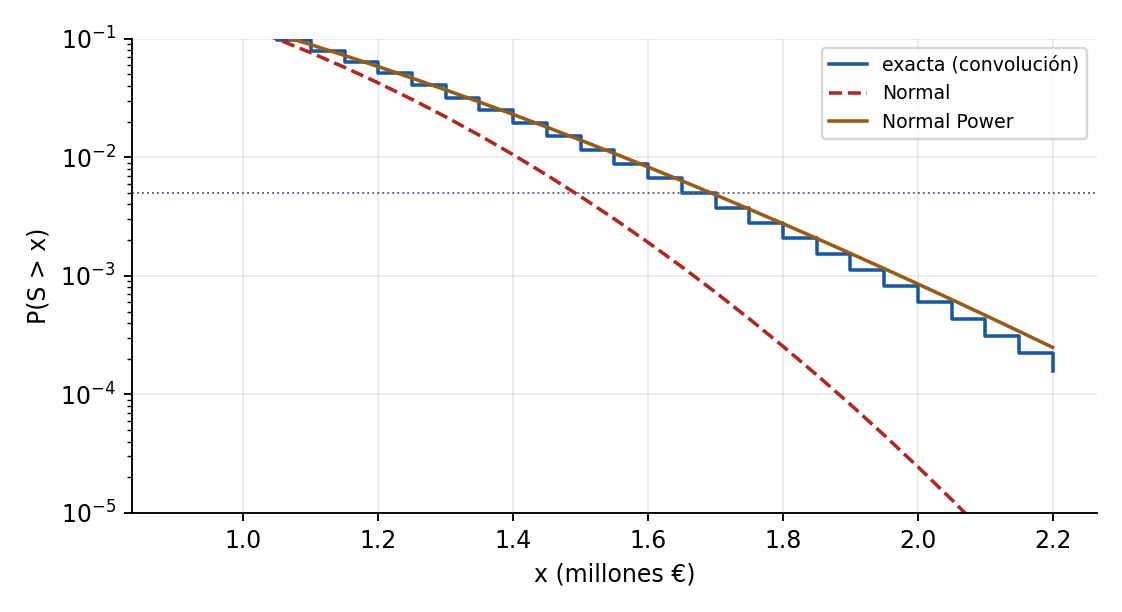
\includegraphics[width=.76\linewidth]{t2_f_repaso2.png}
\caption{Probabilidad de exceder $x$ en la cartera del Caso~1. La Normal cae demasiado deprisa; la Normal Power sigue la cola exacta.}
\end{figure}

\subsection*{Otras razones que se suman}
\begin{itemize}[leftmargin=*,itemsep=1pt]
\item La Normal da probabilidad positiva a siniestralidad negativa y no respeta $S\ge0$ (con asimetr\'ia 4 y $E=10.000$ esa masa es no despreciable).
\item $S$ es discreta o mixta, con masa en $0$; con pocas p\'olizas la distribuci\'on es muy irregular (con 3 p\'olizas del ejemplo $P(S=0)=0{,}94$).
\item La asimetr\'ia baja como $1/\sqrt n$: con 50.000 p\'olizas del mismo perfil la Normal solo se queda un $0{,}6\%$ corta, con 1.000 un $12\%$.
\item Y lo m\'as importante: bajo dependencia (pandemia), no hay convergencia a la Normal; la cola es m\'as gruesa a\'un.
\end{itemize}

\paragraph{Conclusi\'on.} Infravalora porque ignora la asimetr\'ia positiva, y la ignora justo donde se mide el capital. Con tres momentos (Gamma trasladada o Normal Power) el error pasa del $12\%$ a menos del $1\%$.

\bigskip\hrule\bigskip

\section*{Pregunta 3 -- S\'olo hay datos agregados: ?`individual o colectivo?}

\noindent\textbf{Enunciado.} Si una aseguradora solo dispone de datos agregados de siniestralidad (sin desglose por p\'oliza), ?`qu\'e modelo ser\'ia m\'as adecuado, el individual o el colectivo? Justifica la respuesta.

\subsection*{Respuesta: el colectivo}
El modelo individual necesita, para \emph{cada} p\'oliza, la probabilidad $q_i$ y la distribuci\'on de la severidad $(\mu_i,\sigma_i^2)$ o el capital $b_i$. Sin desglose por p\'oliza no hay forma de estimarlos. El modelo colectivo solo necesita lo que s\'i se observa en datos agregados: un modelo para el n\'umero de siniestros $N$ (por ejemplo Poisson o Binomial Negativa, con media estimada del hist\'orico) y una distribuci\'on de la cuant\'ia por siniestro $Y$ (estimada con las cuant\'ias de los siniestros, no de las p\'olizas): $S=\sum_{j=1}^NY_j$.

\subsection*{Matices}
\begin{itemize}[leftmargin=*]
\item \textbf{Qu\'e agregado se tiene.} Si hay datos \emph{por siniestro} (frecuencia y cuant\'ias) aunque no por p\'oliza, el colectivo se estima bien. Si solo se tiene el total anual $S_t$ de unos pocos a\~nos, ni siquiera eso: habr\'ia que ajustar directamente una distribuci\'on a $S$ (por ejemplo Gamma o lognormal) con credibilidad respecto a un benchmark de mercado, y la incertidumbre de par\'ametros ser\'ia grande.
\item \textbf{Equivalencia aproximada.} Para $q_i$ peque\~nas el individual se aproxima por un Poisson compuesto con $\lambda=\sum q_i$ y una severidad mezcla con pesos $q_i/\lambda$. La varianza colectiva es $\sum q_i(\sigma_i^2+\mu_i^2)$ frente a la individual $\sum[q_i\sigma_i^2+q_i(1-q_i)\mu_i^2]$; la diferencia es $\sum q_i^2\mu_i^2\ge0$, as\'i que el colectivo es algo m\'as conservador. En el Caso~1 la varianza colectiva es $1{,}180\cdot10^{11}$ frente a $1{,}172\cdot10^{11}$ ($+0{,}68\%$) y el VaR Normal pasa de $1.491.844$ a $1.494.826$; en la cartera de 8 p\'olizas la diferencia es del $0{,}63\%$. En el Caso~2 (con $q$ entre $0{,}05$ y $0{,}08$) llega al $5{,}3\%$ en varianza y al $1{,}0\%$ en el VaR ($140.049\to141.499$).
\item \textbf{Ventajas pr\'acticas.} Permite recursi\'on de Panjer y FFT, incorpora varios siniestros por p\'oliza, inflaci\'on de severidad y sobredispersi\'on con la Binomial Negativa.
\item \textbf{Lo que se pierde.} El colectivo no ve la heterogeneidad de la cartera: si cambia la mezcla de capitales o de edades (nuevo producto, entrada de grandes riesgos), el modelo estimado deja de ser v\'alido sin reponderarlo, y no sirve para decidir por p\'oliza (suscripci\'on, recargos, reaseguro por riesgo).
\item \textbf{Soluci\'on mixta habitual.} Modelo individual para los grandes riesgos identificables (con $q_i$ y $b_i$ conocidos) y colectivo para el resto (\emph{attritional}).
\end{itemize}

\paragraph{Conclusi\'on.} Con datos solo agregados no cabe el individual; el colectivo es el adecuado, con la cautela de que pierde la informaci\'on de composici\'on de la cartera.

\subsection*{Referencias}
\begin{itemize}[leftmargin=*,itemsep=0pt]
\item Kaas, R., Goovaerts, M., Dhaene, J. y Denuit, M. (2008). \emph{Modern Actuarial Risk Theory} (2.\textordfeminine\ ed.). Springer.
\item De Pril, N. (1986). On the exact computation of the aggregate claims distribution in the individual life model. \emph{ASTIN Bulletin}, 16.
\item Dhaene, J. y De Pril, N. (1994). On a class of approximative computation methods in the individual risk model. \emph{Insurance: Mathematics and Economics}, 14.
\item Klugman, S. A., Panjer, H. H. y Willmot, G. E. \emph{Loss Models: From Data to Decisions}. Wiley.
\end{itemize}
\end{document}
